\documentclass{article}
\PassOptionsToPackage{numbers}{natbib}
\usepackage[preprint]{neurips_2025}
\usepackage[utf8]{inputenc}
\usepackage[T1]{fontenc}
\usepackage{amsmath,amssymb,booktabs,graphicx,url}
\usepackage[hidelinks]{hyperref}
\title{Generating Chest X-Rays with a Convolutional VAE}
\author{Yun-Tong Tsai}
\begin{document}
\maketitle
\begin{abstract}
A PyTorch variational autoencoder (VAE) generates $64\times64$ chest radiographs.
After 30 epochs, Inception Score is 1.697 and torchvision-feature FID is 210.96.
Samples capture coarse chest structure but lack fine detail.
\end{abstract}

\section{Data and model}
Normal and pneumonia images from Kaggle [1] are pooled. SHA-256 deduplication removes
32 files, retaining 618 official test images. Training excludes 453 images
whose filename-derived patient IDs occur in test; 10\% of remaining shuffled groups
form validation (seed 42): 4269 training and 468 validation images.
The 16 official validation images are unused. Preprocessing uses grayscale conversion, PIL bilinear
resize to $64\times64$, and scaling to $[0,1]$, without augmentation; aspect ratios can change.

The encoder uses four $4\times4$ convolutions (stride 2, padding 1; channels
$1,32,64,128,256$; SiLU), then linear heads for 32-dimensional $\mu$ and
$\log\sigma^2$. Reparameterization $z=\mu+\sigma\odot\epsilon$,
$\epsilon\sim\mathcal N(0,I)$, enables backpropagation [2]. A linear projection and
four transposed convolutions reverse these dimensions; sigmoid outputs intensities.
The model has 1,775,361 parameters, without batch normalization.

\section{Training protocol and learning curves}
BCE sums over 4,096 pixels; KL sums over latent dimensions. Minibatch means minimize:
\vspace{-3pt}
\begin{equation}
\mathcal L_\beta=\mathbb E_{q_\phi(z|x)}[-\log p_\theta(x|z)]
+\frac{\beta}{2}\sum_{j=1}^{32}(\mu_j^2+\sigma_j^2-1-\log\sigma_j^2).
\end{equation}
BCE is a soft-target surrogate for continuous intensities. Settings: Adam learning
rate $10^{-3}$, moments $(0.9,0.999)$, batch size 64, zero weight decay, gradient-norm
limit 10, 30 epochs, seed 42, and warm-up $\beta=\min(1,e/5)$ at epoch $e$.
Validation uses fixed posterior noise and $\beta=1$; its minimum selects epoch
30 (2391.81 nats/image).
\begin{figure}[h]
\centering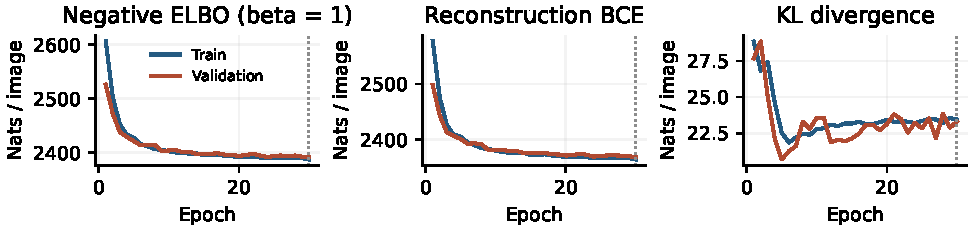
\includegraphics[width=\linewidth]{loss_curves.pdf}
\caption{Losses per image; the left panel uses $\beta=1$ even during warm-up.
Training values average across updates; dotted lines mark the selected checkpoint.}
\end{figure}
\newpage
\section{Generation and quantitative evaluation}
The selected decoder generates 618 prior samples from $z\sim\mathcal N(0,I)$
(seed 123), compared with all 618 test images using Ignite's FID/IS evaluator [3].
Both sets receive 8-bit conversion, RGB replication, PIL bilinear resize to
$299\times299$, and ImageNet normalization (an addition to the tutorial).
Frozen torchvision Inception-v3 (\texttt{IMAGENET1K\_V1}) supplies 2,048 pooled
features for the primary FID and 1,000 softmax probabilities for IS and the
Ignite-default FID representation. Neither FID is comparable to TensorFlow-weight
\texttt{pytorch-fid} scores. Generated images are sigmoid decoder means, with no visual selection.

\begin{table}[h]
\centering
\caption{Test results at epoch 30. Losses: nats/image. Split IS reports mean
and standard deviation over ten subsets, not independently trained models.}
\begin{tabular}{lr@{\qquad}lr}
\toprule
Metric & Value & Metric & Value \\
\midrule
FID (2,048 pool features)$\downarrow$ & 210.96 & Test negative ELBO$\downarrow$ & 2391.06 \\
FID (1,000 probabilities)$\downarrow$ & 0.28299 & Test reconstruction BCE$\downarrow$ & 2367.58 \\
IS (all samples)$\uparrow$ & 1.697 & Test KL & 23.47 \\
IS (10 splits)$\uparrow$ & $1.677\pm0.080$ & Real / generated count & 618 / 618 \\
\bottomrule
\end{tabular}
\end{table}
\begin{figure}[h]
\centering
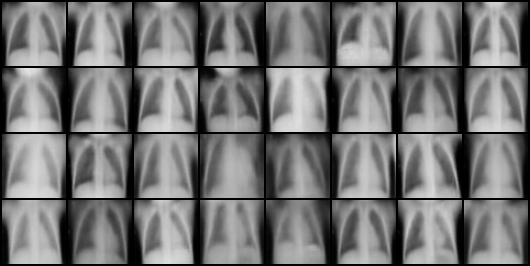
\includegraphics[width=.76\linewidth]{generated.png}
\caption{The first 32 generated images from evaluation seed 123, in order.
All panels use the same $[0,1]$ display range.}
\end{figure}

\section{Discussion and limitations}
Validation negative ELBO decreases from 2,525.63 at epoch 1 to 2,391.81 at epoch 30, while the final training value is 2,387.57. The small gap provides no clear evidence of overfitting in this run. Generated samples capture broad lung fields and a central bright region, with variation in width and intensity, but fine structures are blurred and some boundaries are distorted. The nonzero test KL indicates that the posterior differs from the prior; it alone does not prove that every latent dimension is useful. Pixelwise reconstruction and the low spatial resolution likely contribute to the limited detail.
Filename grouping cannot verify clinical identity or near-duplicates.
With only 618 test images, the 2,048-feature covariance is rank deficient and
FID is affected by finite-sample bias. ImageNet-based IS cannot establish pathology
coverage or anatomical correctness. Only one training and sampling seed are evaluated.
Higher resolution, repeated runs, and radiograph-specific evaluation are useful next steps.

\small
\begin{thebibliography}{3}
\setlength{\itemsep}{0pt}
\bibitem{data} P. Mooney. \href{https://www.kaggle.com/datasets/paultimothymooney/chest-xray-pneumonia}{\emph{Chest X-Ray Images (Pneumonia)}}. Kaggle.
\bibitem{vae} D. P. Kingma and M. Welling. Auto-Encoding Variational Bayes. ICLR, 2014.
\href{https://arxiv.org/abs/1312.6114}{arXiv:1312.6114}.
\bibitem{ignite} PyTorch-Ignite. \href{https://pytorch-ignite.ai/blog/gan-evaluation-with-fid-and-is/}{GAN evaluation using FID and IS}.
\end{thebibliography}
\end{document}
